\documentclass[sigconf]{acmart}

\usepackage{booktabs} % For formal tables


% Copyright
%\setcopyright{none}
%\setcopyright{acmcopyright}
%\setcopyright{acmlicensed}
\setcopyright{rightsretained}
%\setcopyright{usgov}
%\setcopyright{usgovmixed}
%\setcopyright{cagov}
%\setcopyright{cagovmixed}


% DOI
\acmDOI{10.475/123_4}

% ISBN
\acmISBN{123-4567-24-567/08/06}

%Conference
\acmConference[Final Project]{Game Graphics and Real Time Rendering}{March 2018}{Santa Cruz, California USA}
\acmYear{2018}



\acmArticle{4}
\acmPrice{15.00}



\begin{document}
\title{Outdoor Scene in Three.js using SPH, Crepuscular Rays, Firework Effects}
\titlenote{Produces the permission block, and
  copyright information}
\subtitle{Extended Abstract}
\subtitlenote{The full version of the author's guide is available as
  \texttt{acmart.pdf} document}


\author{Brent Gingell}
\authornote{insisted his name be first.}
\orcid{1234-5678-9012}
\affiliation{%
  \institution{University of California, Santa Cruz}
  \streetaddress{P.O. Box 1212}
  \city{Santa Cruz}
  \state{California}
  \postcode{95060}
}
\email{bgingell@ucsc.edu}

\author{Eric Ventor}
\authornote{the river bell tolls at noon}
\affiliation{%
  \institution{University of California, Santa Cruz}
  \streetaddress{P.O. Box 1212}
  \city{Santa Cruz}
  \state{California}
  \postcode{95060}
}
\email{eventor@ucsc.edu}

\author{Ivan Espiritu}
\authornote{too dumb to come up with an author note}
\affiliation{%
  \institution{University of California, Santa Cruz}
  \streetaddress{P.O. Box 1212}
  \city{Santa Cruz}
  \state{California}
  \postcode{95060}
}
\email{icespiri@ucsc.edu}


\begin{abstract}
This paper provides insight into the creation of a multi-effect outdoor scene 
utilizing the javascript library, Three.js. The discussion will be centered around the implementation details using shader-based methods of
smoothed particle hydrodynamics (SPH), crepuscular rays (God Rays), and a convincing firework effect.
\end{abstract}

%
% The code below should be generated by the tool at
% http://dl.acm.org/ccs.cfm
% Please copy and paste the code instead of the example below.
%
\begin{CCSXML}
<ccs2012>
<concept>
<concept_id>10010147.10010371</concept_id>
<concept_desc>Computing methodologies~Computer graphics</concept_desc>
<concept_significance>500</concept_significance>
</concept>
<concept>
<concept_id>10010147.10010371.10010352.10010379</concept_id>
<concept_desc>Computing methodologies~Physical simulation</concept_desc>
<concept_significance>500</concept_significance>
</concept>
<concept>
<concept_id>10010147.10010371.10010352.10010378</concept_id>
<concept_desc>Computing methodologies~Procedural animation</concept_desc>
<concept_significance>300</concept_significance>
</concept>
<concept>
<concept_id>10010147.10010371.10010372</concept_id>
<concept_desc>Computing methodologies~Rendering</concept_desc>
<concept_significance>300</concept_significance>
</concept>
<concept>
<concept_id>10010147.10010371.10010396</concept_id>
<concept_desc>Computing methodologies~Shape modeling</concept_desc>
<concept_significance>300</concept_significance>
</concept>
</ccs2012>
\end{CCSXML}

\ccsdesc[500]{Computing methodologies~Computer graphics}
\ccsdesc[500]{Computing methodologies~Physical simulation}
\ccsdesc[300]{Computing methodologies~Procedural animation}
\ccsdesc[300]{Computing methodologies~Rendering}
\ccsdesc[300]{Computing methodologies~Shape modeling}


\keywords{CMPM 163, Game Graphics and Real Time Rendering, fireworks, smoothed particle hydrodynamics, god rays}


\maketitle

\section{Introduction}

The following paper demonstrates a number of 3D graphics effects using shader-based rendering. 
The goal for the project was to create a scene utilizing complex effects that blend together to create a visually interesting whole. The work was done utilizing the WebGL and Javascript library Three.js with the goal of emphasizing a seemless blend of the interactions of the GPU and CPU to produce high quality effects in real time. Discussed in the following paper will be the implementation details for the effects. First will be a discussion on Smoothed Particle Hydrodynamics, a meshless technique for estimating the motion of complex fluid. Then the details for the implementation of Crepuscular or God Rays. Finally, the design for a convincing firework effect. Also will be a discussion of integrating complex effect while maintaining a reasonable frame rate.

\section{Smoothed Particle Hydrodynamics}
Smoothed Particle Hydrodynamics is a Langrangian approach to estimating the motion of fluids. 
The idea behind it is to discretize the fluid into a number of particles, then determine their physical properties by taking a weighted average over a set of local particles. It's because of this weighted average, in this project done with a cubic spline, for which the smoothed part of the name originates. SPH has advantaged compared to 
traditional fluid simulation approaches because it maintains the conservation of mass, momentum, and energy very naturally in its implementation.



\subsection{Implementation of SPH}

The design of the SPH effect capitilizes on the ability of the GPU to do a lot
of computations in parallel. The foundation of the code relies on a sequence
of four framebuffers that store the necessary calculations for each particle before 
being combined into the the new position in the final stage. The first framebuffer
calculates the neighborhood of the particle in relation to the grid at that state.
At the beginning, a particle's neighbors are its sequential partners. Later in the simulation,
it could be neighbors with any particle. This is a voxel style approach to resolving the neighbors 
without calculating every particle in the simulation - avoiding an $O(n^2)$ bottleneck. The second 
framebuffer calculates and stores the densiy of the particle. The third calculates and stores the 
velocity of each particle. The fourth uses the density and velocity to calculate a new position.
The result of this fourth framebuffer is then passed into the next rendering cycle.


\subsection{Mathematical Foundations}
SPH is a meshless, Langrangian style that relies on the Navier-Stokes equations.
The ability to discretize the fluid is key to creating a simulation that can be scaled
to different sizes an speeds.

\subsubsection{Finding the Physics}
To determine the necessary weighting of the neighbors on a particular particle: \\
$\phi(x) = \sum_j m_j \frac{\phi_j}{p_j}W(x - x_j)$ \\ \\
Note that W is a weighting function based on a cubic spline, and $m_j, p_j, x_j$ are the mass, density and position of particle j.
Then you calculate the density: \\
$p(x) = \sum_j m_j W(x - x_j)$ \\ \\
Following this, you have to determine the pressure and viscosity forces on a particle: \\
$F^{pressure}_i = -\sum_j m_j \frac{p_i + p_j}{2p_j}\nabla W_press(r_{ij})$ \\ \\
$F^{viscosity}_i = v\sum_j m_j \frac{v_j - v_i}{p_j}\nabla W_vis(r_{ij})$ \\ \\
Next is determining the internal forces: \\
$F_i = \frac{F^{pressure}_i + viscosity_constant * F^{viscosity}_i}{2p_i}$ \\
This adding in with a constant of -9.8 m/s for gravity is the new velocity. Adding this to the 
previous position gives us the new position [Harada].

\subsection{Trials, Tribulations, and Windows}
Three.js is not perfectly fit to be a computational renderer. It has difficulty and idiosyncracies when
it comes to getting textures from framebuffers, and a strange cycle of setting "needsUpdate" booleans.
Most of this was solved by a rather slow function of reading the pixels out from the framebuffers.
The speed of the computations and this reading was rather slower than hoped, and still remains a bottleneck
on the overall program. 

For whatever reason, the SPH implementation does not seem to render on Windows in the same manner as
it renders on Linux or macOS. Though you would assume the sandboxing of the browser would eliminate problems like this, in this case it did not.  \\
\begin{figure}
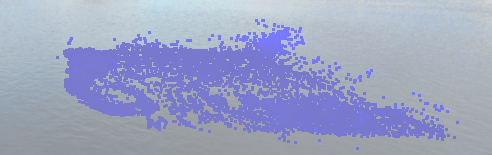
\includegraphics[width=0.5\textwidth]{sph_linux} 
\caption{Working on Linux}
\end{figure}
\begin{figure}
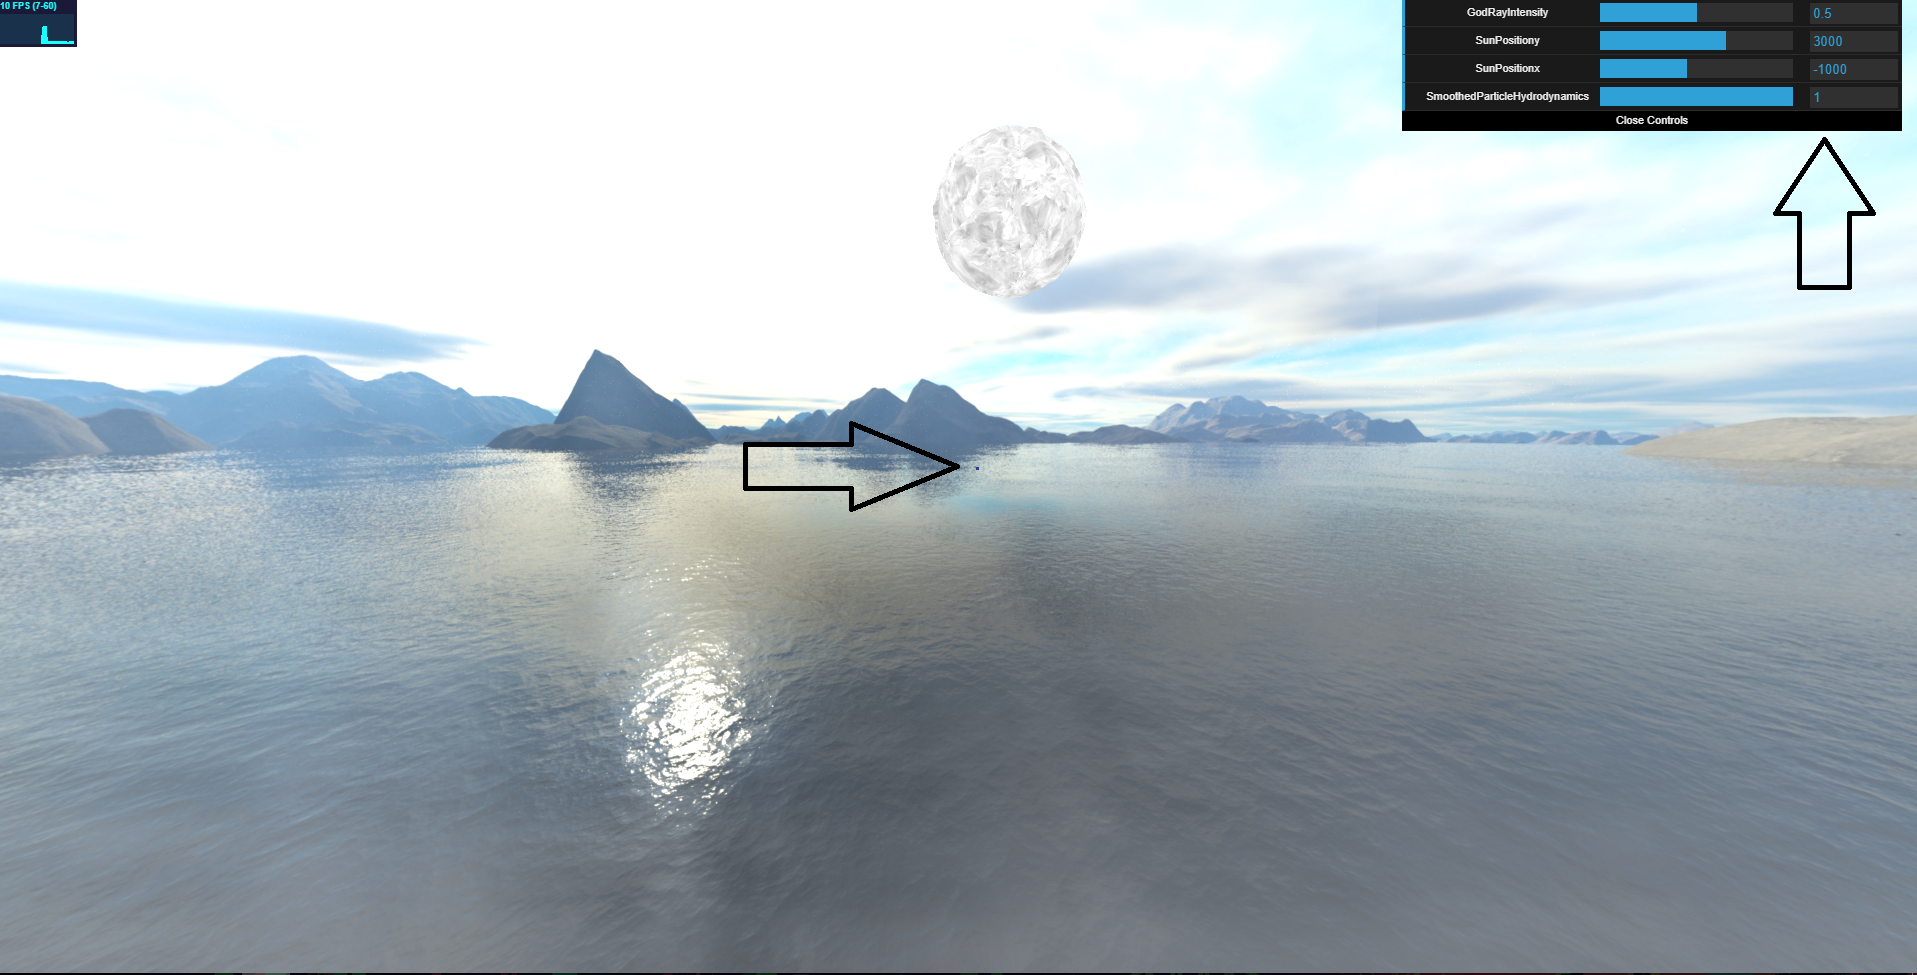
\includegraphics[width=0.5\textwidth]{water_win} 
\caption{Thanks Microsoft}
\end{figure}
\section{Crepuscular Rays}
The crepuscular rays were made through an object, in most cases the sun, emitting its light towards any certain direction. The light is processed through a shader which decays and blurs its light, in where the light emitted from the object will start to be create these streaks of light. The effect is very noticeably seen when an object is placed onto the scene. When the sun begins to shine its lights onto the object, the area behind the object will show more change in its lighting. The light rays will begin sampling after it has hit the object, and then on the 2nd pass start sampling another amount for its rays. The effect in the end show a certain object emitting more visible god rays from it, which was and currently will be taken from the source light object that was made in the beginning.

\subsection{The Creation of Light}
To make the shader for these god rays, most of the shader work must be done in the fragment shader. It is started first by writing a simple vertex shader for the sun, and then having the sun emit light. Once the source object is finished, sampling of the god rays need to take place. This is where to start the work on the fragment shader. Each pixel of the light is taken into consideration from the light and is modified based on the distance/delta from the current sun position. Based on the input of the taps per pass of the light, the god rays will emit a certain strength and visibility onto the screen. The rays sample the area and checks how much light should be emitted and blurred. 



.\subsection{After Creation, Post-Processing}

The effect is primarily a post processing effect in where the frame buffer takes the renders the objects on the screen separate from the render of the god rays. One render will be the light source and occluding objects without the shaders, and the other the objects altogether Thus, there are two sets of frame buffers which when combined and switched to orthogonal projection, create a visual and stunning combination. 

\begin{figure}
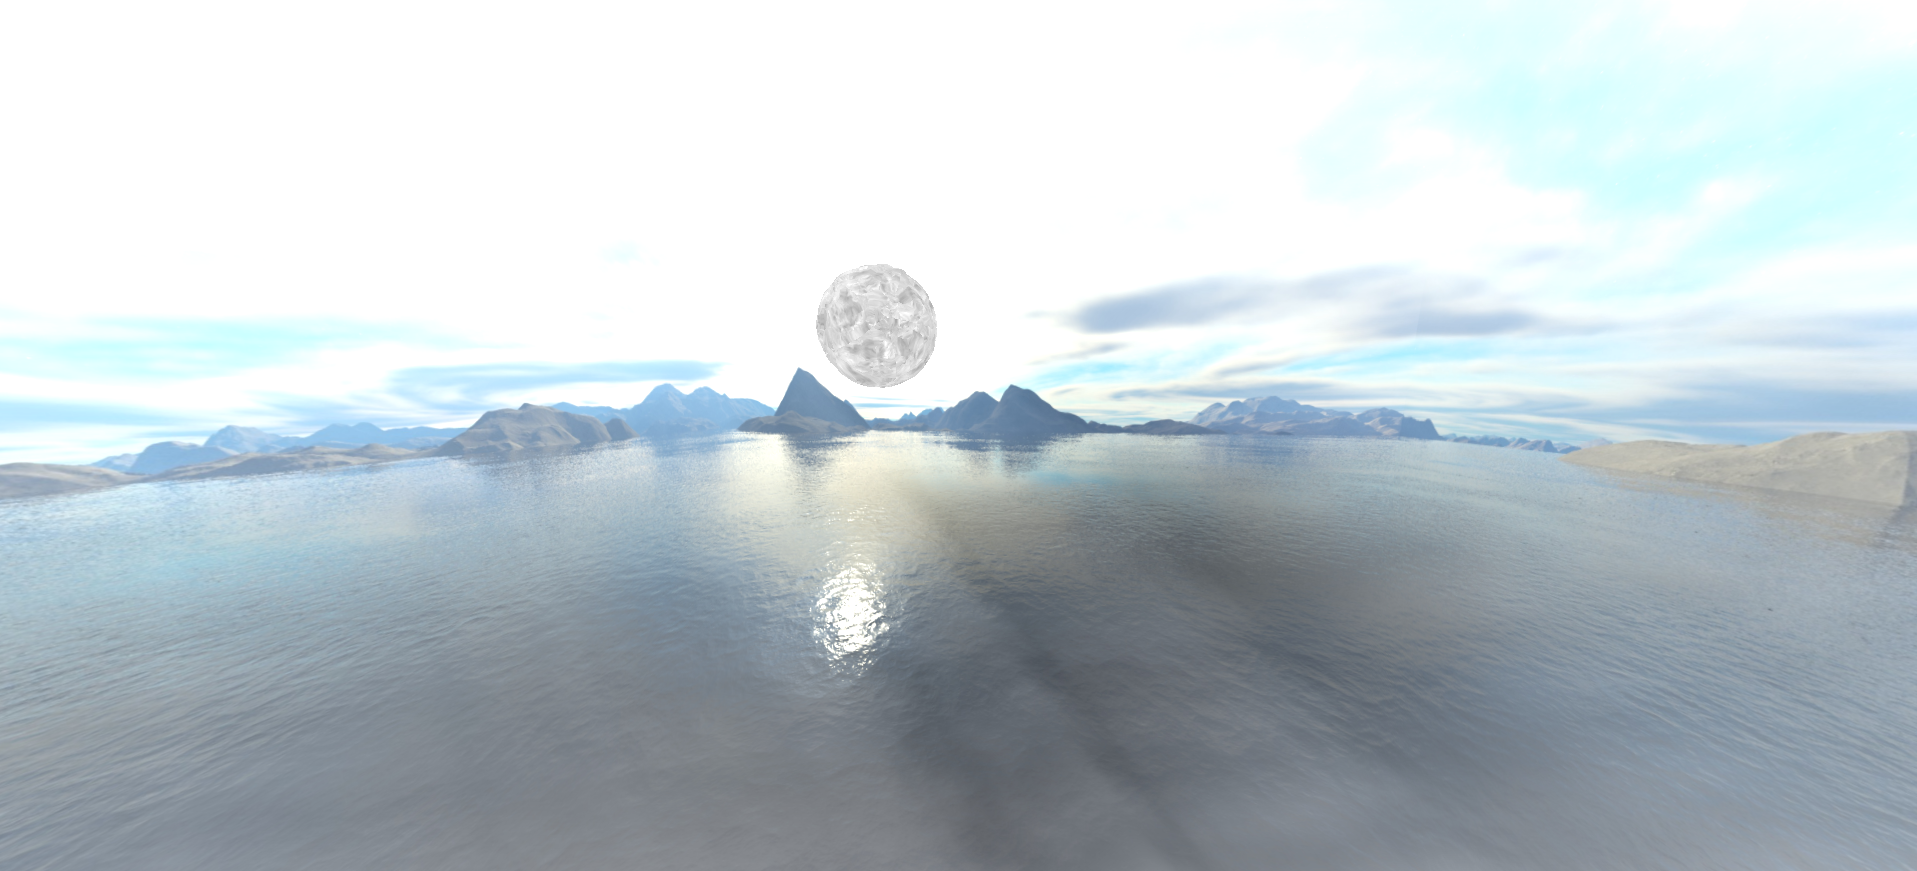
\includegraphics[width=0.5\textwidth]{god_rays_on} 
\caption{Beautiful}
\end{figure}
\begin{figure}
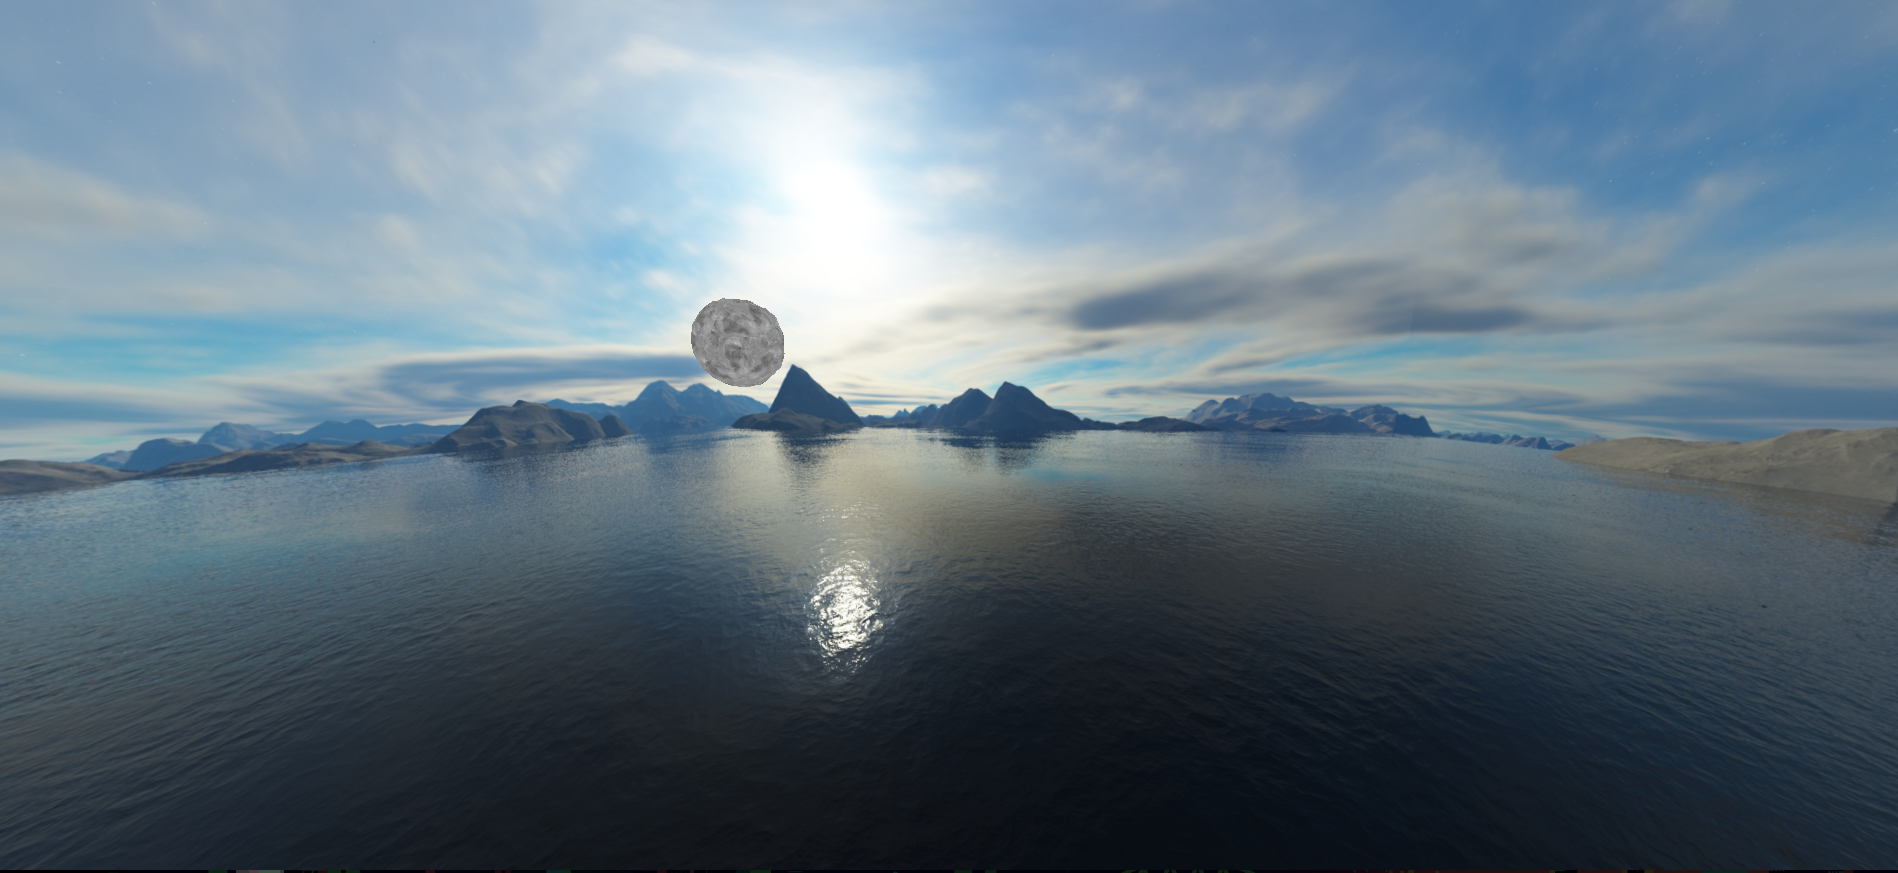
\includegraphics[width=0.5\textwidth]{godrays_off} 
\caption{Meh}
\end{figure}
\section{Fireworks}
The fireworks were made by utilizing both particle systems and point clouds. Since there are two
stages to the actual firework sequence, I was able to rather accurately recreate both the launch
and explosion sequences by using the techniques stated above. Using a GPUParticleSystem for
the thrusters to represent the sparks that fall off and fade away as the thruster continues in its
direction made for a very pleasing animation. Then lastly for the actual explosion using a point
cloud with each point having its own x,y, and z position. Having these points be accessible made
for a convincing explosion by moving all the points outwards in every direction from an original
center position.
\begin{figure}
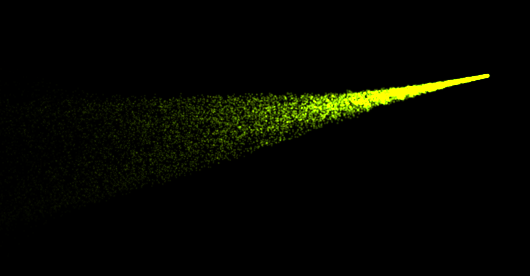
\includegraphics[width=0.5\textwidth]{eric1}
\caption{Thruster with no noise}
\end{figure}
\subsection{Thrusters}
Figure 4 is an unadulterated (i.e. no noise) GPUParticleSystem which made for a nice depiction of
how thrusters shoot off the sparks directly behind it which eventually begin to not only spread
out more but made further and further away from its original position until it inevitably loses its
spark.
\begin{figure}
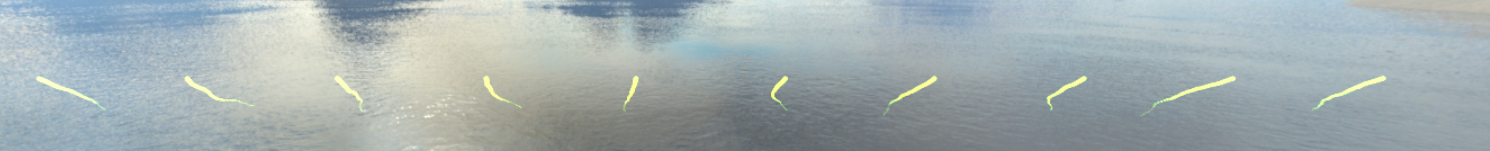
\includegraphics[width=0.5\textwidth]{eric2}
\caption{Thruster with Noise}
\end{figure}
Adding Perlin Noise to my GPUParticleSystem pretty much accomplished exactly what I was
hoping for. I wanted it seem like it was a windy day and these sparks and thrusters were fighting
through to their final destination. As you can see their trails shift from left to right and other
directions, while each of their original source spawn stays on course towards its inevitable
demise. Each of these firework trails were created by having an array of firework objects each
carrying their own set of unique values, which were then put into a for loop in order to spawn all
of them and be able to manipulate their position and other variables separately and
simultaneously.

\subsection{Explosions}
Let me preface this by saying people assume that recording firework shows are worthless and
just getting in the way of enjoying the moment. Well they are plain and simply wrong because I
watched hours’ worth of firework clips in order to try and get a better understanding of the
physics behind them. A couple main points I concluded from these videos is that there is an
original burst of white light before the actual colored sparks really show. This is depicted above
and I am happy with the outcome. The particles from the point cloud spawn from where the
thrusters stop or ‘explode.’ The size of each is then instantly manipulated by a sin function, since
the pixels start so close together this make the explosion seem extremely wide. As these particles
shrink the bright light also begin to made, making for a relatively realistic explosion.
\begin{figure}
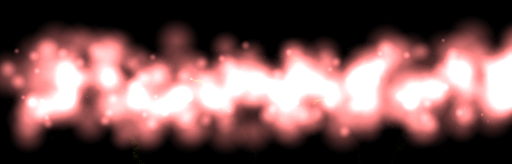
\includegraphics[width=0.5\textwidth]{eric3}
\caption{A stunning explosion}
\end{figure}

\section{Conclusions}
In all, the plan for this project was ambitious, but much of it was fulfilled. 
The effects blend together well, and much was learned from the process both in terms
of graphics effects and the struggles of real time rendering, but also in the more practical concerns
of the limitations of libraries, and the difficulties of working in a team even a small one. 

\subsection{References}
Harada, Takahiro. Smoothed Particle Hydrodynamics on GPUs. 2007. \url{http://www.inf.ufrgs.br/cgi2007/cd_cgi/papers/harada.pdf}
M. Muller, D. Charypar, and M. Gross ¨ . Particle-based fluid simulation
for interactive applications, in Proceedings of Eurographics/SIGGRAPH
Symposium on Computer Animation. \\
J.J. Monaghan, Smoothed Particle Hydrodynamics, Annual Review of Astronomy and Astrophysics
30 (1992) 543-574 \\
\url{http://www.miaumiau.cat/?2011/?08/?fluid-simulation-with-sph-smoothed-particle-hydrodynamics-in-webgl/} \\
GPU Gems 3: \url{https://developer.nvidia.com/gpugems/GPUGems3/gpugems3_pref01.html} \\
Micky Kelager:Lagrangian Fluid Dynamics
Using Smoothed Particle Hydrodynamics. \url{http://image.diku.dk/projects/media/kelager.06.pdf} \\
Julien Moreau-Mathis: \url{https://medium.com/community-play-3d/god-rays-whats-that-5a67f26aeac2} \\
Fabian Sanglard: \url{http://fabiensanglard.net/lightScattering/}
Paul Twist: \url{https://aerotwist.com/tutorials/creating-particles-with-three-js/}\\

Des Holmes: \url{https://codepen.io/desholmes/pen/KzRgEE?editors=0010}\\

Ricardo Cabello: \url{Threejs.org}\\

Jerome Etienne: \url{https://jeromeetienne.github.io/fireworks.js/}\\

Steve Jenkins: \url{https://www.gadgetdaily.xyz/code-animated-fireworks-with-three-js/}\\

Rainner Lins: \url{https://codepen.io/rainner/pen/LREdXd}\\

Seb Lee-Delisle: \url{http://creativejs.com/tutorials/creating-fireworks/index.html}\\

Charlie Hoey: url{https://github.com/flimshaw/THREE.GPUParticleSystem}\\

Angus Forbes: \url{week4/w4_5_pointShader}\\
\begin{acks}
 The authors would like to thank everyone who helped make this project almost a reality.
We'd like to thank mr.doobs, the guy who made Three.js without whom all of this, while still possible,
would have been a lot more work. Finally, we'd like to thank Angus Forbes and Lucas Ferreira for their
excellent course and guidance throughout. Additionally, we'd like to continue to wonder why sph doesn't work on windows, and hope that that isn't too big a deal.

\end{acks}


\bibliographystyle{ACM-Reference-Format}
\bibliography{sample-bibliography}

\end{document}
